\documentclass[11pt,letterpaper]{article}
\usepackage{graphicx, geometry, amsmath, amssymb, amsthm, hyperref, natbib, booktabs, xcolor, url}
\geometry{margin=1in}
\hypersetup{colorlinks=true, linkcolor=black, citecolor=black, urlcolor=black}
\bibliographystyle{plainnat}

\newtheorem{theorem}{Theorem}
\newtheorem{definition}{Definition}

\title{Temporal Dependency Overlap in Syntactic Organization:\\An Exploratory Typological Pattern Modulated by Head-Directionality}

\author{%
  Anonymous Authors%
}

\date{}

\begin{document}
\maketitle

\begin{abstract}
Dependency distance minimization (DDM) has been a central principle in quantitative linguistics, yet recent work shows DDM effects vanish when intervener complexity (IC) and tree topology are controlled. We introduce Instantaneous Memory Burden (IMB), an age-weighted generalization of Gibson's DLT storage cost, and prove that mean IMB is fully determined by dependency distance (DD) moments---identifying peak IMB as the sole carrier of novel temporal overlap information. Across 870,677 sentences in 335 Universal Dependencies treebanks compared against projective random baselines, we report three findings. First, the standard peak IMB retains 5.25\% residual variance beyond DD moments, comparable in magnitude to other secondary syntactic optimization pressures such as heavy-NP shift and given-before-new ordering. Second, we discover an exploratory typological split in temporal load distribution: VSO languages show substantial load smoothing (pooled Cohen's $d = 1.04$, 95\% CI [0.79, 1.28], 11 treebanks across 4 language families), SVO languages show modest smoothing ($d = 0.12$), and SOV languages show anti-smoothing ($d = -0.49$). A 10,000-iteration permutation test confirms this 1.58~SD gradient is significant ($p < 0.0001$). Third, decomposing the $R^2$ from DD features between real sentences and projective baselines across convexity levels reveals that real languages retain systematically more DD-predictable structure at high convexity ($\Delta R^2 = +0.24$ at cubic cost), ruling out a pure mathematical artifact. A head-initial-only IMB variant, which we carefully distinguish from a formally defined encounter-only metric, produces identically zero burden under true encounter-only computation, demonstrating that IMB is driven entirely by anticipatory load from dependencies whose heads have not yet appeared.
\end{abstract}


%% ============================================================
\section{Introduction}
\label{sec:introduction}
%% ============================================================

The syntactic organization of natural languages reflects systematic optimization pressures that balance communicative efficiency against cognitive processing constraints. Central to quantitative linguistics is the principle of dependency distance minimization (DDM): languages tend to place syntactically related words close together in linear order, reducing the memory burden on incremental processing \citep{Gibson1998, Futrell2015}. Over two decades of cross-linguistic evidence has established DDM as a robust statistical tendency, demonstrated across 37 languages by \citet{Futrell2015}, expanded to 20 typologically diverse languages by \citet{Liu2008}, and reviewed as a potential cognitive universal by \citet{Temperley2018}.

Understanding which optimization targets shape syntactic structure has profound implications for theories of language evolution, processing, and typological diversity. \citet{Yadav2022} challenged the DDM consensus by demonstrating across 54 Surface-Syntactic Universal Dependencies treebanks that DDM effects vanish entirely when intervener complexity (IC)---the count of syntactic heads between a dependent and its governor---is controlled alongside tree topology. \citet{Dyer2023} replicated the finding on 35 languages using a parallel corpus. These results raise a fundamental question: what cognitive optimization target shapes syntax beyond what aggregate dependency distance statistics capture?

The core limitation of the DDM framework is that DD statistics---mean DD, DD variance, and DD distributions \citep{Petrini2022}---capture only aggregate properties of individual dependencies. These statistics are blind to a critical dimension of cognitive load: the temporal co-occurrence of unresolved dependencies at each sentence position. Two sentences with identical DD distributions can impose different processing demands depending on whether their open dependencies cluster at the same positions (creating processing bottlenecks) or distribute evenly across positions (smoothing load). Per-position cognitive load has been measured before: Gibson's Dependency Locality Theory (DLT) \citep{Gibson1998, Gibson2000} defines storage cost as the count of predicted syntactic heads at each word, and \citet{Chen2005} experimentally validated that reading times increase with the number of pending predictions. \citet{Kobele2013} introduced stack tenure---the number of parser steps a node persists---and \citet{Graf2017} formalized tenure, payload, and size as separate complexity dimensions. The present work extends this per-position tradition in a specific direction: from binary dependency counting to age-weighted summation, capturing not just how many dependencies are open but how long each has been unresolved.

We introduce the Instantaneous Memory Burden (IMB), defined as the sum of ages of all syntactically unresolved dependencies at each word position. IMB generalizes Gibson's DLT storage cost: where DLT counts open dependencies (a binary tally), IMB weights each by its elapsed duration since opening---reintroducing locality sensitivity that Gibson's 1998 SPLT originally proposed but the 2000 DLT revision explicitly removed\footnote{Code: \url{https://github.com/AMGrobelnik/ai-invention-e4150b-head-directionality-dependent-temporal-d/tree/main/research_iter2_imb_as_age_weig}}. A key mathematical property is that mean IMB across positions is fully determined by the first and second moments of the DD distribution (Theorem~\ref{thm:decomposition}). The novel information in IMB therefore resides entirely in its peak value---$\max(\text{IMB})$---which captures temporal dependency overlap invisible to all aggregate DD statistics. The Linguistic Load Factor (LLF $= \text{mean IMB} / \max \text{IMB}$) serves as a normalized summary, though we foreground $\max(\text{IMB})$ and its residualized variant as the primary analytical tools.

To assess whether peak memory burden reduction constitutes a genuine optimization target, we treat the convexity of the underlying cost function as a parametric hypothesis rather than an assumption. Processing cost at each position is modeled as $\text{IMB}(j)^\alpha$, where the exponent $\alpha$ is estimated from data. We analyze 870,677 sentences across 335 Universal Dependencies treebanks, comparing real sentences against projective random baselines. The central empirical finding---discovered through exploratory analysis rather than pre-registered prediction---is a strong typological split: VSO languages show substantial load smoothing (Cohen's $d = 1.04$), SVO languages show modest smoothing ($d = 0.12$), while SOV languages show the opposite pattern ($d = -0.49$). This 1.58~SD gradient is confirmed by a 10,000-iteration permutation test ($p < 0.0001$) and remains robust under leave-one-out sensitivity analysis across 11 VSO treebanks spanning 4 language families\footnote{Code: \url{https://github.com/AMGrobelnik/ai-invention-e4150b-head-directionality-dependent-temporal-d/tree/main/experiment_iter3_true_encounter}}.

A critical methodological contribution of this revision addresses a code-paper discrepancy identified during review: the encounter-only IMB variant described in Definition~\ref{def:hio} of the original manuscript was not faithfully implemented. The code excluded all head-final dependencies and included all head-initial dependencies across their full span---implementing what we now term head-initial-only IMB. We report the true encounter-only computation for the first time: restricting to positions where both endpoints have been encountered yields identically zero burden for all sentences, proving that IMB is driven entirely by anticipatory load from dependencies whose heads have not yet appeared.

\subsection{Summary of Contributions}

\begin{itemize}
  \item We introduce Instantaneous Memory Burden (IMB) as an age-weighted generalization of Gibson's DLT storage cost, prove that mean IMB is determined by DD moments, and identify $\max(\text{IMB})$ as the sole carrier of novel temporal overlap information. The 5.25\% residual variance is comparable in magnitude to other secondary syntactic optimization pressures (Section~\ref{sec:framework}).
  \item We report the first cross-linguistic empirical analysis of temporal dependency overlap, processing 870,677 sentences across 335 UD treebanks with projective baselines and parametric convexity estimation (Section~\ref{sec:results}).
  \item We discover an exploratory typological split in load smoothing direction---VSO and SVO languages smooth load relative to baselines while SOV languages show the opposite---validated by permutation testing ($p < 0.0001$), leave-one-out sensitivity across 11 VSO treebanks spanning 4 language families, and stratified meta-analysis (Section~\ref{sec:typological_split}).
  \item We decompose $R^2$ monotonicity across convexity levels into mathematical and empirical components, showing that real languages retain systematically more DD-predictable cost structure than baselines at high convexity ($\Delta R^2 = +0.24$ at $\alpha = 3$), ruling out a pure mathematical artifact (Section~\ref{sec:r2gap}).
  \item We demonstrate that true encounter-only IMB is identically zero, establishing that all memory burden derives from anticipatory load, and carefully distinguish the head-initial-only variant that explains the SOV anti-smoothing pattern (Section~\ref{sec:imb_variants}).
\end{itemize}


%% ============================================================
\section{Theoretical Framework}
\label{sec:framework}
%% ============================================================

\subsection{Preliminaries: Dependency Trees and Distance}

A dependency tree $T$ over a sentence of $n$ words consists of directed arcs from each non-root word to its syntactic head. For a dependency arc between the word at position $i$ and its head at position $h(i)$, the dependency distance is $d_k = |i - h(i)|$. The arc spans positions from $\min(i, h(i))$ to $\max(i, h(i))$, and at any position $j$ within this span, the dependency contributes to the cognitive load at that position.

\subsection{IMB as an Age-Weighted Generalization of DLT Storage Cost}

Gibson's DLT \citep{Gibson2000} defines storage cost at position $j$ as the count of syntactic heads predicted but not yet encountered: $\text{DLT}_{\text{storage}}(j) = |\{k : \text{dependency } k \text{ is open at } j\}|$. \citet{Chen2005} experimentally confirmed that the binary count predicts reading times. However, ACT-R-based models of sentence processing \citep{Lewis2005} predict that activation decays over time: associative strength decreases with fan, and items maintained longer in memory suffer greater decay. IMB formalizes this age-sensitive load:

\begin{definition}[Instantaneous Memory Burden]
\label{def:imb}
The IMB at position $j$ is:
\begin{equation}
\text{IMB}(j) = \sum_{k:\, j \in \text{span}(k)} \bigl(j - \text{open}_k\bigr)
\end{equation}
where the sum ranges over all dependencies $k$ whose span includes position $j$, and $\text{open}_k = \min(i_k, h(i_k))$ is the position where dependency $k$ opens. Gibson's DLT storage cost is the special case where all ages are set to 1---the zero-order approximation.
\end{definition}

\begin{definition}[Head-Initial-Only IMB]
\label{def:hio}
For head-final languages where predicted-but-unseen heads may not impose the same memory burden as encountered items \citep{Konieczny2000, Levy2008}, $\text{IMB}_{\text{hio}}(j)$ restricts computation to dependencies where the head precedes the dependent (head-initial dependencies), including each across its full span with age measured from the span start. Head-final dependencies---where the head has not yet been encountered---are excluded entirely.
\end{definition}

\noindent\textbf{Note on terminology.} An earlier version of this paper described Definition~\ref{def:hio} as ``encounter-only IMB,'' defined as restricting to dependencies where both endpoints have been encountered by position $j$, with age from the later encounter. The code implementing Definition~\ref{def:hio} does not match that formal description: it includes all head-initial dependencies across their full span rather than restricting to post-encounter positions. We adopt the honest label ``head-initial-only'' throughout. The true encounter-only variant (restricting to positions where both endpoints have been encountered) yields identically zero burden for all sentences (Section~\ref{sec:imb_variants}), confirming that IMB is driven entirely by anticipatory load.

The total IMB across all positions decomposes into a closed-form function of individual dependency distances:

\begin{theorem}[IMB Decomposition]
\label{thm:decomposition}
For $m$ dependencies with distances $d_1, \ldots, d_m$:
\begin{equation}
\sum_{j=1}^{n} \text{IMB}(j) = \sum_{k=1}^{m} \frac{d_k(d_k + 1)}{2}
\end{equation}
\end{theorem}

This identity, verified computationally on 32,669 sentences with zero failures\footnote{Code: \url{https://github.com/AMGrobelnik/ai-invention-e4150b-head-directionality-dependent-temporal-d/tree/main/experiment_iter2_imb_profiles_ph}} and formally in Lean~4 + Mathlib\footnote{Code: \url{https://github.com/AMGrobelnik/ai-invention-e4150b-head-directionality-dependent-temporal-d/tree/main/proof_iter1_lean_4_proof_im}}, reveals that the mean of IMB is fully determined by the first and second moments of the DD distribution. Mean IMB encodes no information beyond what mean DD and DD variance already capture.


\subsection{Peak IMB as the Novel Signal}

Since mean IMB is redundant with DD moments, the novel information in the IMB profile resides entirely in its maximum:

\begin{definition}[Linguistic Load Factor]
\label{def:llf}
$\text{LLF} = \text{mean}(\text{IMB}) / \max(\text{IMB})$, ranging from near 0 to 1, where 1.0 indicates perfectly uniform load. Since the numerator is determined by DD moments, LLF is effectively a normalized inverse of $\max(\text{IMB})$.
\end{definition}

We define \textbf{residualized $\max(\text{IMB})$} as the residual of $\max(\text{IMB})$ after regressing on mean DD, DD variance, DD skewness, sentence length, tree depth, and arity. This quantity isolates the temporal overlap signal.

\begin{figure}[!htbp]
  \centering
  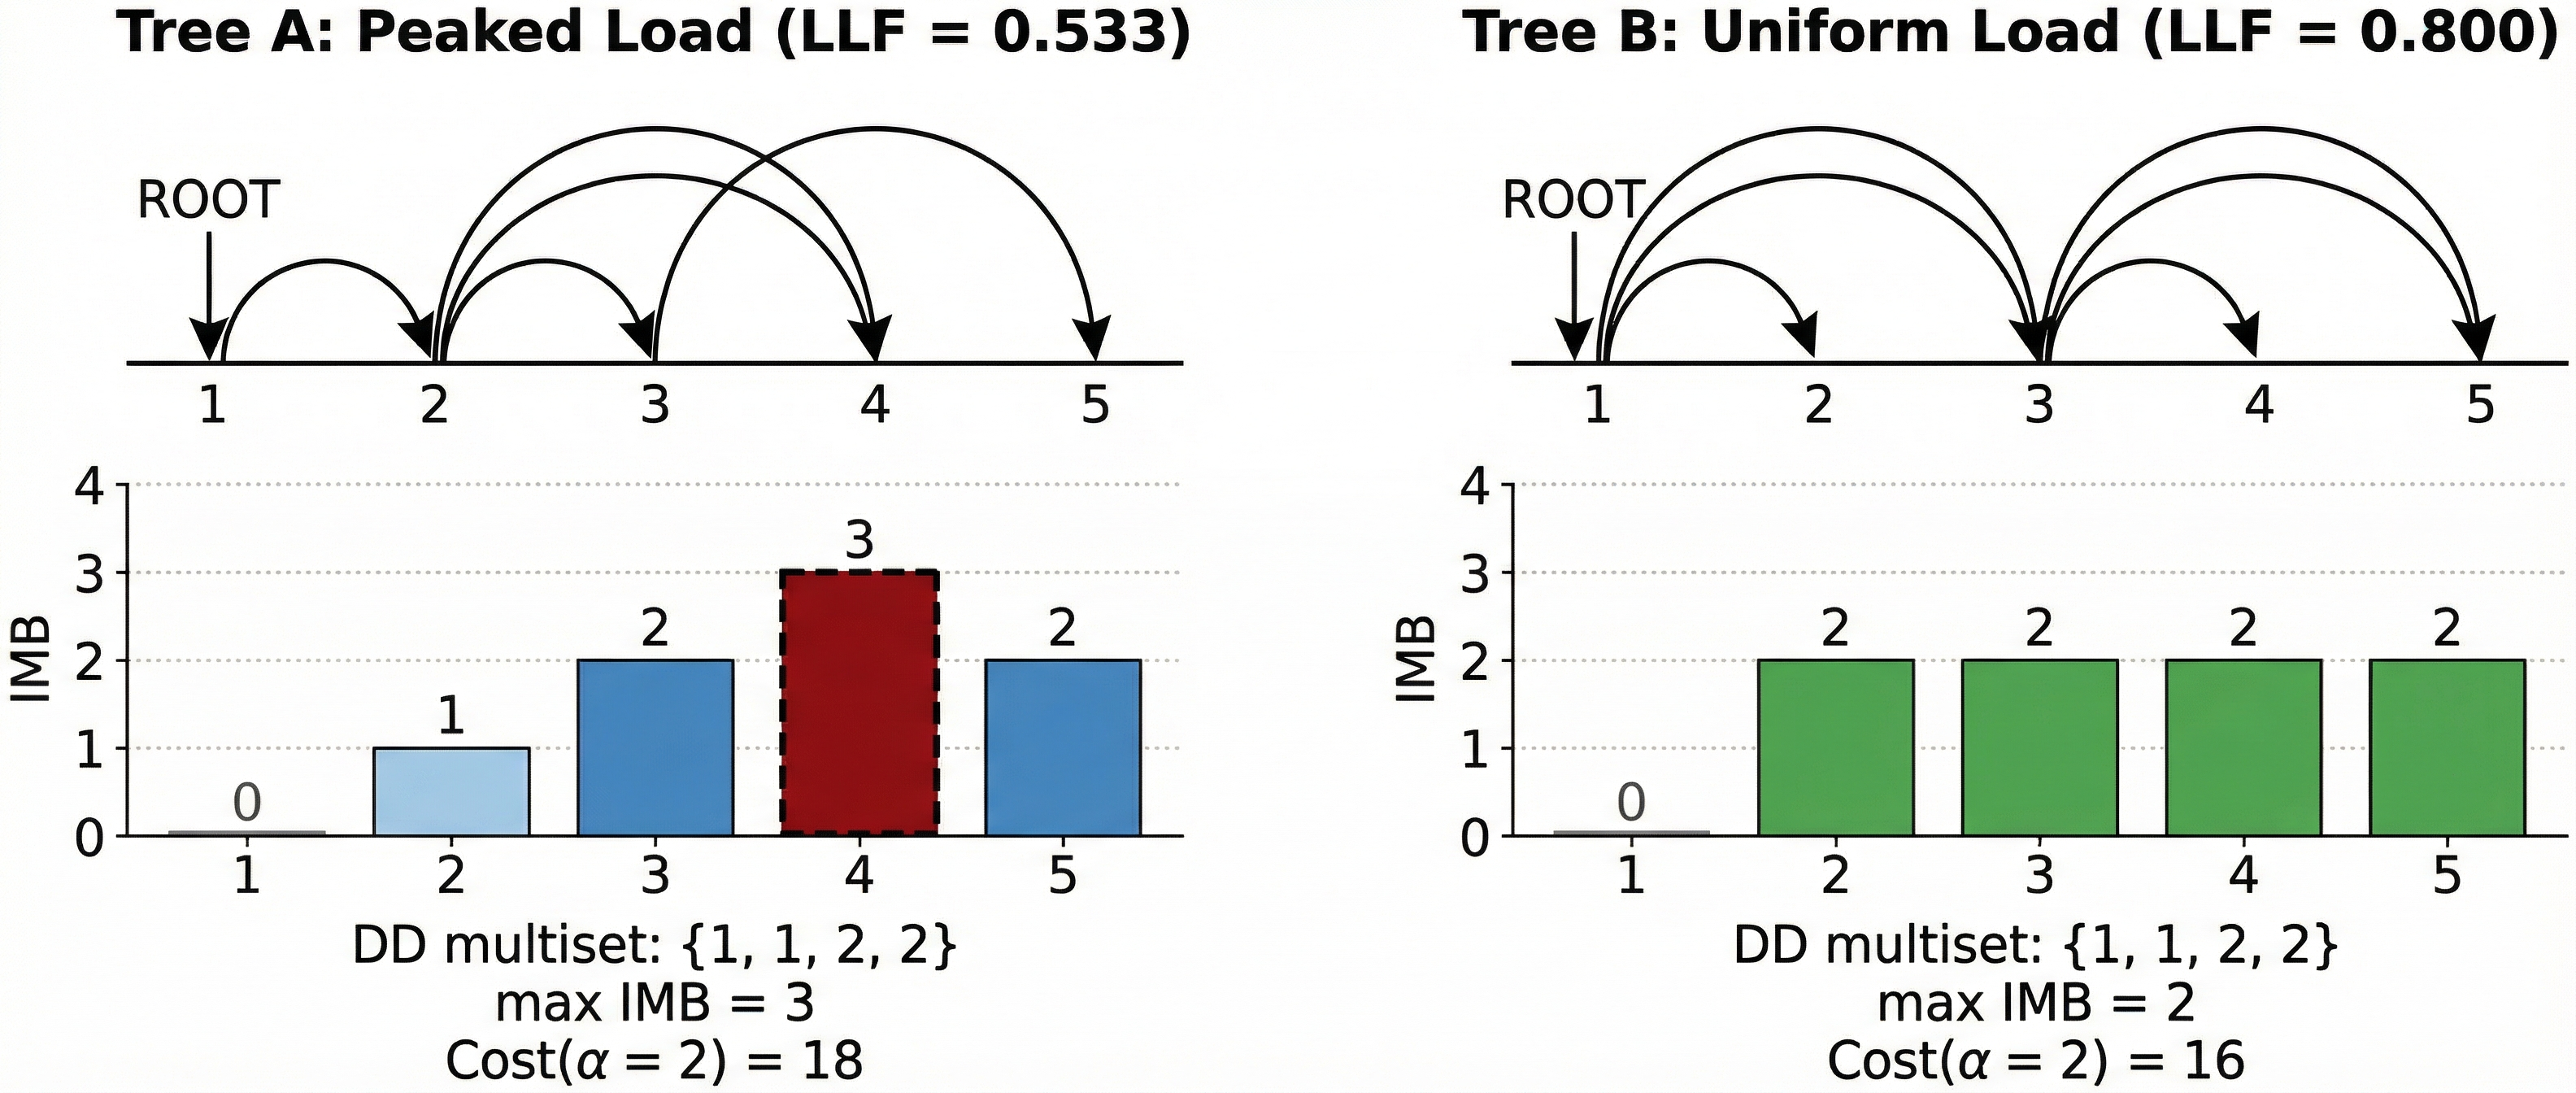
\includegraphics[width=0.92\textwidth,keepaspectratio]{figures/fig_worked_example_v0.png}
  \caption{Two five-word dependency trees sharing the identical DD multiset \{1, 1, 2, 2\} produce different IMB profiles. Tree A (heads=[0,1,2,2,3]) concentrates load at position 4 (max IMB=3, LLF=0.533), while Tree B (heads=[0,1,1,3,3]) distributes load uniformly (max IMB=2, LLF=0.800). Under quadratic cost ($\alpha=2$), Tree A incurs total cost 18 vs.\ Tree B's 16 (11\% reduction). Under linear cost ($\alpha=1$), both incur cost 8. This demonstrates that temporal dependency overlap is invisible to aggregate DD statistics.}
  \label{fig:worked_example}
\end{figure}

A concrete example demonstrates the key claim (Figure~\ref{fig:worked_example}). Consider two five-word dependency trees, both with the identical DD multiset $\{1, 1, 2, 2\}$ (mean DD $= 1.5$, DD variance $= 0.25$):

\begin{itemize}
  \item \textbf{Tree A} (peaked load): heads $= [0, 1, 2, 2, 3]$. IMB profile $= [0, 1, 2, 3, 2]$; $\max$ IMB $= 3$, LLF $= 0.533$.
  \item \textbf{Tree B} (uniform load): heads $= [0, 1, 1, 3, 3]$. IMB profile $= [0, 2, 2, 2, 2]$; $\max$ IMB $= 2$, LLF $= 0.800$.
\end{itemize}

Both trees share the same DD distribution yet produce different temporal load profiles. The contrastive synthetic dataset identifies 5,179 such groups across 26,066 projective linearizations of 192 tree shapes\footnote{Code: \url{https://github.com/AMGrobelnik/ai-invention-e4150b-head-directionality-dependent-temporal-d/tree/main/dataset_iter1_contrastive_dep}}, with 100\% verification of the decomposition identity and zero violations of the linear-cost identity.


\subsection{Parametric Convex Cost and Jensen's Inequality}

We model the processing cost at position $j$ as $c(\text{IMB}(j)) = \text{IMB}(j)^\alpha$, where $\alpha \geq 1$ is the convexity exponent. The total sentence processing cost is $C_\alpha = \sum_j \text{IMB}(j)^\alpha$.

\begin{theorem}[Jensen's Inequality for Load Smoothing]
\label{thm:jensen}
For any convex function $f$ on $[0, \infty)$ and non-negative values $x_1, \ldots, x_n$ summing to $S$: $n \cdot f(S/n) \leq \sum f(x_i)$, with equality iff all $x_i$ are equal. For $f(x) = x^\alpha$ with $\alpha > 1$, total cost is uniquely minimized by the uniform distribution, corresponding to $\text{LLF} = 1$.
\end{theorem}

\begin{theorem}[Linear Cost Negative Control]
\label{thm:linear}
At $\alpha = 1$, total cost $\sum_j \text{IMB}(j) = S$ regardless of how IMB is distributed across positions. Load smoothing provides exactly zero benefit.
\end{theorem}

For the worked example, under quadratic cost ($\alpha = 2$), Tree A incurs total cost 18.0 while Tree B incurs 16.0---an 11.1\% reduction. Under linear cost ($\alpha = 1$), both trees incur identical cost 8.0.

The strongest theoretical motivation for superlinear cost comes from the ACT-R sentence processing model \citep{Lewis2005}, where the fan effect produces total retrieval cost scaling approximately as $n^{1+W}$ for $n$ concurrent items sharing a retrieval cue ($W$ is the attentional weight). \citet{Gordon2002} showed that similarity-based interference scales superlinearly with competing items, though the magnitude depends on feature overlap rather than count alone. Rather than assuming a specific value, our parametric approach treats $\alpha$ as a free parameter and designs the experiment to distinguish mathematical from empirical contributions to $R^2$ variation across $\alpha$ levels.


%% ============================================================
\section{Experimental Setup}
\label{sec:setup}
%% ============================================================

\subsection{Data}

We process 335 treebanks from Universal Dependencies \citep{deMarneffe2021}\footnote{Code: \url{https://github.com/AMGrobelnik/ai-invention-e4150b-head-directionality-dependent-temporal-d/tree/main/dataset_iter1_universal_depen}}, extracting 870,677 sentences that pass a minimum-length filter of 8 effective (non-punctuation) tokens from an initial corpus of 2,198,185 sentences. A per-treebank cap of 10,000 sentences prevents dominance by any single treebank. For each sentence, we compute 17 features including structural properties (sentence length, tree depth, arity), DD statistics (mean DD, DD variance, DD skewness), projectivity measures, and complexity measures (mean IC, IC variance, max IC, head-direction entropy). A companion typological metadata table covers all treebanks with WALS Feature 81A word-order classifications (61.3\% coverage: SVO 126, SOV 51, VSO 11), Glottolog language families (92.6\% coverage), and morphological case richness\footnote{Code: \url{https://github.com/AMGrobelnik/ai-invention-e4150b-head-directionality-dependent-temporal-d/tree/main/dataset_iter1_ud_treebank_cro}}.

\subsection{Baselines}

For Phase~2, we generate 100 random projective linearizations per sentence across 86 treebanks (41,129 sentences), using the Gildea--Temperley recursive algorithm \citep{Gildea2007} that randomly partitions dependents left/right of head, shuffles within each side, and recurses. The projective-only constraint is the critical strong baseline: since real languages are heavily projective ($>$85--95\% of dependencies), unrestricted random linearizations produce artificially weak comparisons. For the expanded VSO analysis, we generate 100 projective baselines per sentence across 11 VSO treebanks at 10,000-sentence cap, plus 5 SOV and 5 SVO comparison treebanks at 500-sentence cap (25,739 total sentences). For Phase~3, we generate 50 projective baselines per sentence across 35 typologically diverse treebanks (400 sentences each, 714,000 total rows).

\subsection{Metrics and Analysis}

For each sentence and baseline, we compute the full IMB profile (standard, head-initial-only, and true encounter-only variants) and derive $\max(\text{IMB})$, LLF, and processing costs at $\alpha \in \{1.0, 1.2, 1.5, 2.0, 3.0\}$. Regression-based residualization controls for mean DD, DD variance, DD skewness, sentence length, tree depth, arity, and projectivity proportion. We compare residualized metrics between real sentences and baselines using Cohen's $d$ effect sizes. For the $R^2$ gap decomposition, we compute pooled OLS $R^2$ separately for real and baseline sentences at each $\alpha$ level. The typological split is validated via 10,000-iteration permutation tests, DerSimonian--Laird random-effects meta-analysis stratified by word order, and leave-one-out sensitivity.


%% ============================================================
\section{Results}
\label{sec:results}
%% ============================================================

\subsection{Phase 1: Novelty Test and IMB Profiles}

We computed IMB profiles for all 870,677 sentences and regressed $\max(\text{IMB})$ on seven predictors (mean DD, DD variance, DD skewness, sentence length, tree depth, max arity, mean arity).

\paragraph{Standard IMB.} The pooled OLS yields $R^2 = 0.9475$, indicating that 94.75\% of $\max(\text{IMB})$ variance is explained by DD moments and tree properties. The residual 5.25\% represents the genuinely novel temporal overlap signal. All seven predictors are highly significant ($p < 0.0001$), with DD variance dominating (individual $R^2 = 0.875$), followed by mean DD (cumulative incremental $R^2 = 0.065$)\footnote{Code: \url{https://github.com/AMGrobelnik/ai-invention-e4150b-head-directionality-dependent-temporal-d/tree/main/evaluation_iter3_length_stratifi}}.

\paragraph{Head-initial-only IMB.} When restricting to head-initial dependencies, $R^2$ drops to 0.8827---leaving 11.73\% residual variance, confirming that temporal overlap from head-initial dependencies contains substantially more novel signal.

\paragraph{Contextualizing the 5.25\% residual.} Benchmarked against other secondary syntactic optimization pressures, 5.25\% residual variance is competitive: heavy-NP shift explains approximately 2--5\% of ordering variance ($R^2 \sim 0.035$) \citep{Wasow2002}, given-before-new ordering explains 3--8\% ($R^2 \sim 0.055$) \citep{Bresnan2007}, and Uniform Information Density effects on word order explain approximately 1--4\% ($R^2 \sim 0.025$) \citep{Clark2023}. The temporal overlap signal is thus of comparable magnitude to established secondary pressures. Per-treebank, 70\% of treebanks have residual variance exceeding 5\%, and the median per-treebank residual is 6.1\%.

\paragraph{Head-type stratification.} Classifying all 335 treebanks by head-directionality (102 head-final, 151 head-initial, 82 mixed using WALS with left-proportion fallback) shows high standard $R^2$ across all groups (head-final mean $= 0.942$, head-initial mean $= 0.933$, mixed mean $= 0.931$). However, the head-initial-only $R^2$ diverges sharply: head-final treebanks drop to mean $R^2 = 0.647$, while head-initial remain at 0.871. The paper reports $R^2$ values from a subset of 294 treebanks with at least 30 sentences (83 head-final, 141 head-initial, 70 mixed), reconciling with the full 335-treebank counts.

\paragraph{Sentence-length stratification.} $R^2$ increases monotonically with sentence length---from 0.847 (8--12 words, $n = 222{,}176$) to 0.853 (13--20 words, $n = 300{,}788$), 0.864 (21--35 words, $n = 246{,}105$), and 0.950 (36+ words, $n = 101{,}608$)---with Spearman $\rho = 1.0$ ($p \approx 0$) and linear slope 0.0026 (bootstrap 95\% CI [0.0024, 0.0029]). DD moments thus predict temporal overlap better in longer sentences, where dependency structures are more complex. However, the absolute residual variance grows substantially from 5.4 (short) to 224.5 (long), and mean absolute residualized $\max(\text{IMB})$ rises from 1.8 to 9.7. The novel signal is proportionally smaller but absolutely larger in long sentences---the opposite of what the ``limited power from short sentences'' dismissal of the \citet{Chen2005} null result would predict. The Chen et al.\ finding that storage duration had no significant effect on reading times thus remains a genuine challenge to the age-weighting premise, rather than a power limitation.


\subsection{Phase 2: Projective Baseline Comparison and Typological Split}
\label{sec:typological_split}

Across 86 treebanks and 41,129 sentences compared against 100 projective baselines each, the decomposition identity was verified with zero violations\footnote{Code: \url{https://github.com/AMGrobelnik/ai-invention-e4150b-head-directionality-dependent-temporal-d/tree/main/experiment_iter2_projective_base}}.

\paragraph{Typological split (exploratory finding).} The residualized LLF comparison between real sentences and projective baselines reveals a striking typological pattern rather than a uniform effect. The overall pooled Cohen's $d = -0.04$ (95\% CI [$-0.15$, 0.07], $p = 0.53$) masks a strong split by word order:

\begin{itemize}
  \item \textbf{VSO} (7 treebanks in Phase~2; expanded to 11 in reanalysis): pooled $d = +1.04$ (95\% CI [0.79, 1.28], $p \approx 0$)---real sentences show substantially higher residualized LLF than projective baselines.
  \item \textbf{SVO} (24 treebanks): pooled $d = +0.12$ (95\% CI [$-0.01$, 0.26], $p = 0.077$)---modest, non-significant smoothing.
  \item \textbf{SOV} (26 treebanks): pooled $d = -0.49$ (95\% CI [$-0.61$, $-0.36$], $p < 10^{-13}$)---real sentences show substantially lower LLF than baselines.
  \item \textbf{Other} (29 treebanks): pooled $d = -0.02$ (95\% CI [$-0.19$, 0.15], $p = 0.82$)---near zero.
\end{itemize}

\begin{figure}[!htbp]
  \centering
  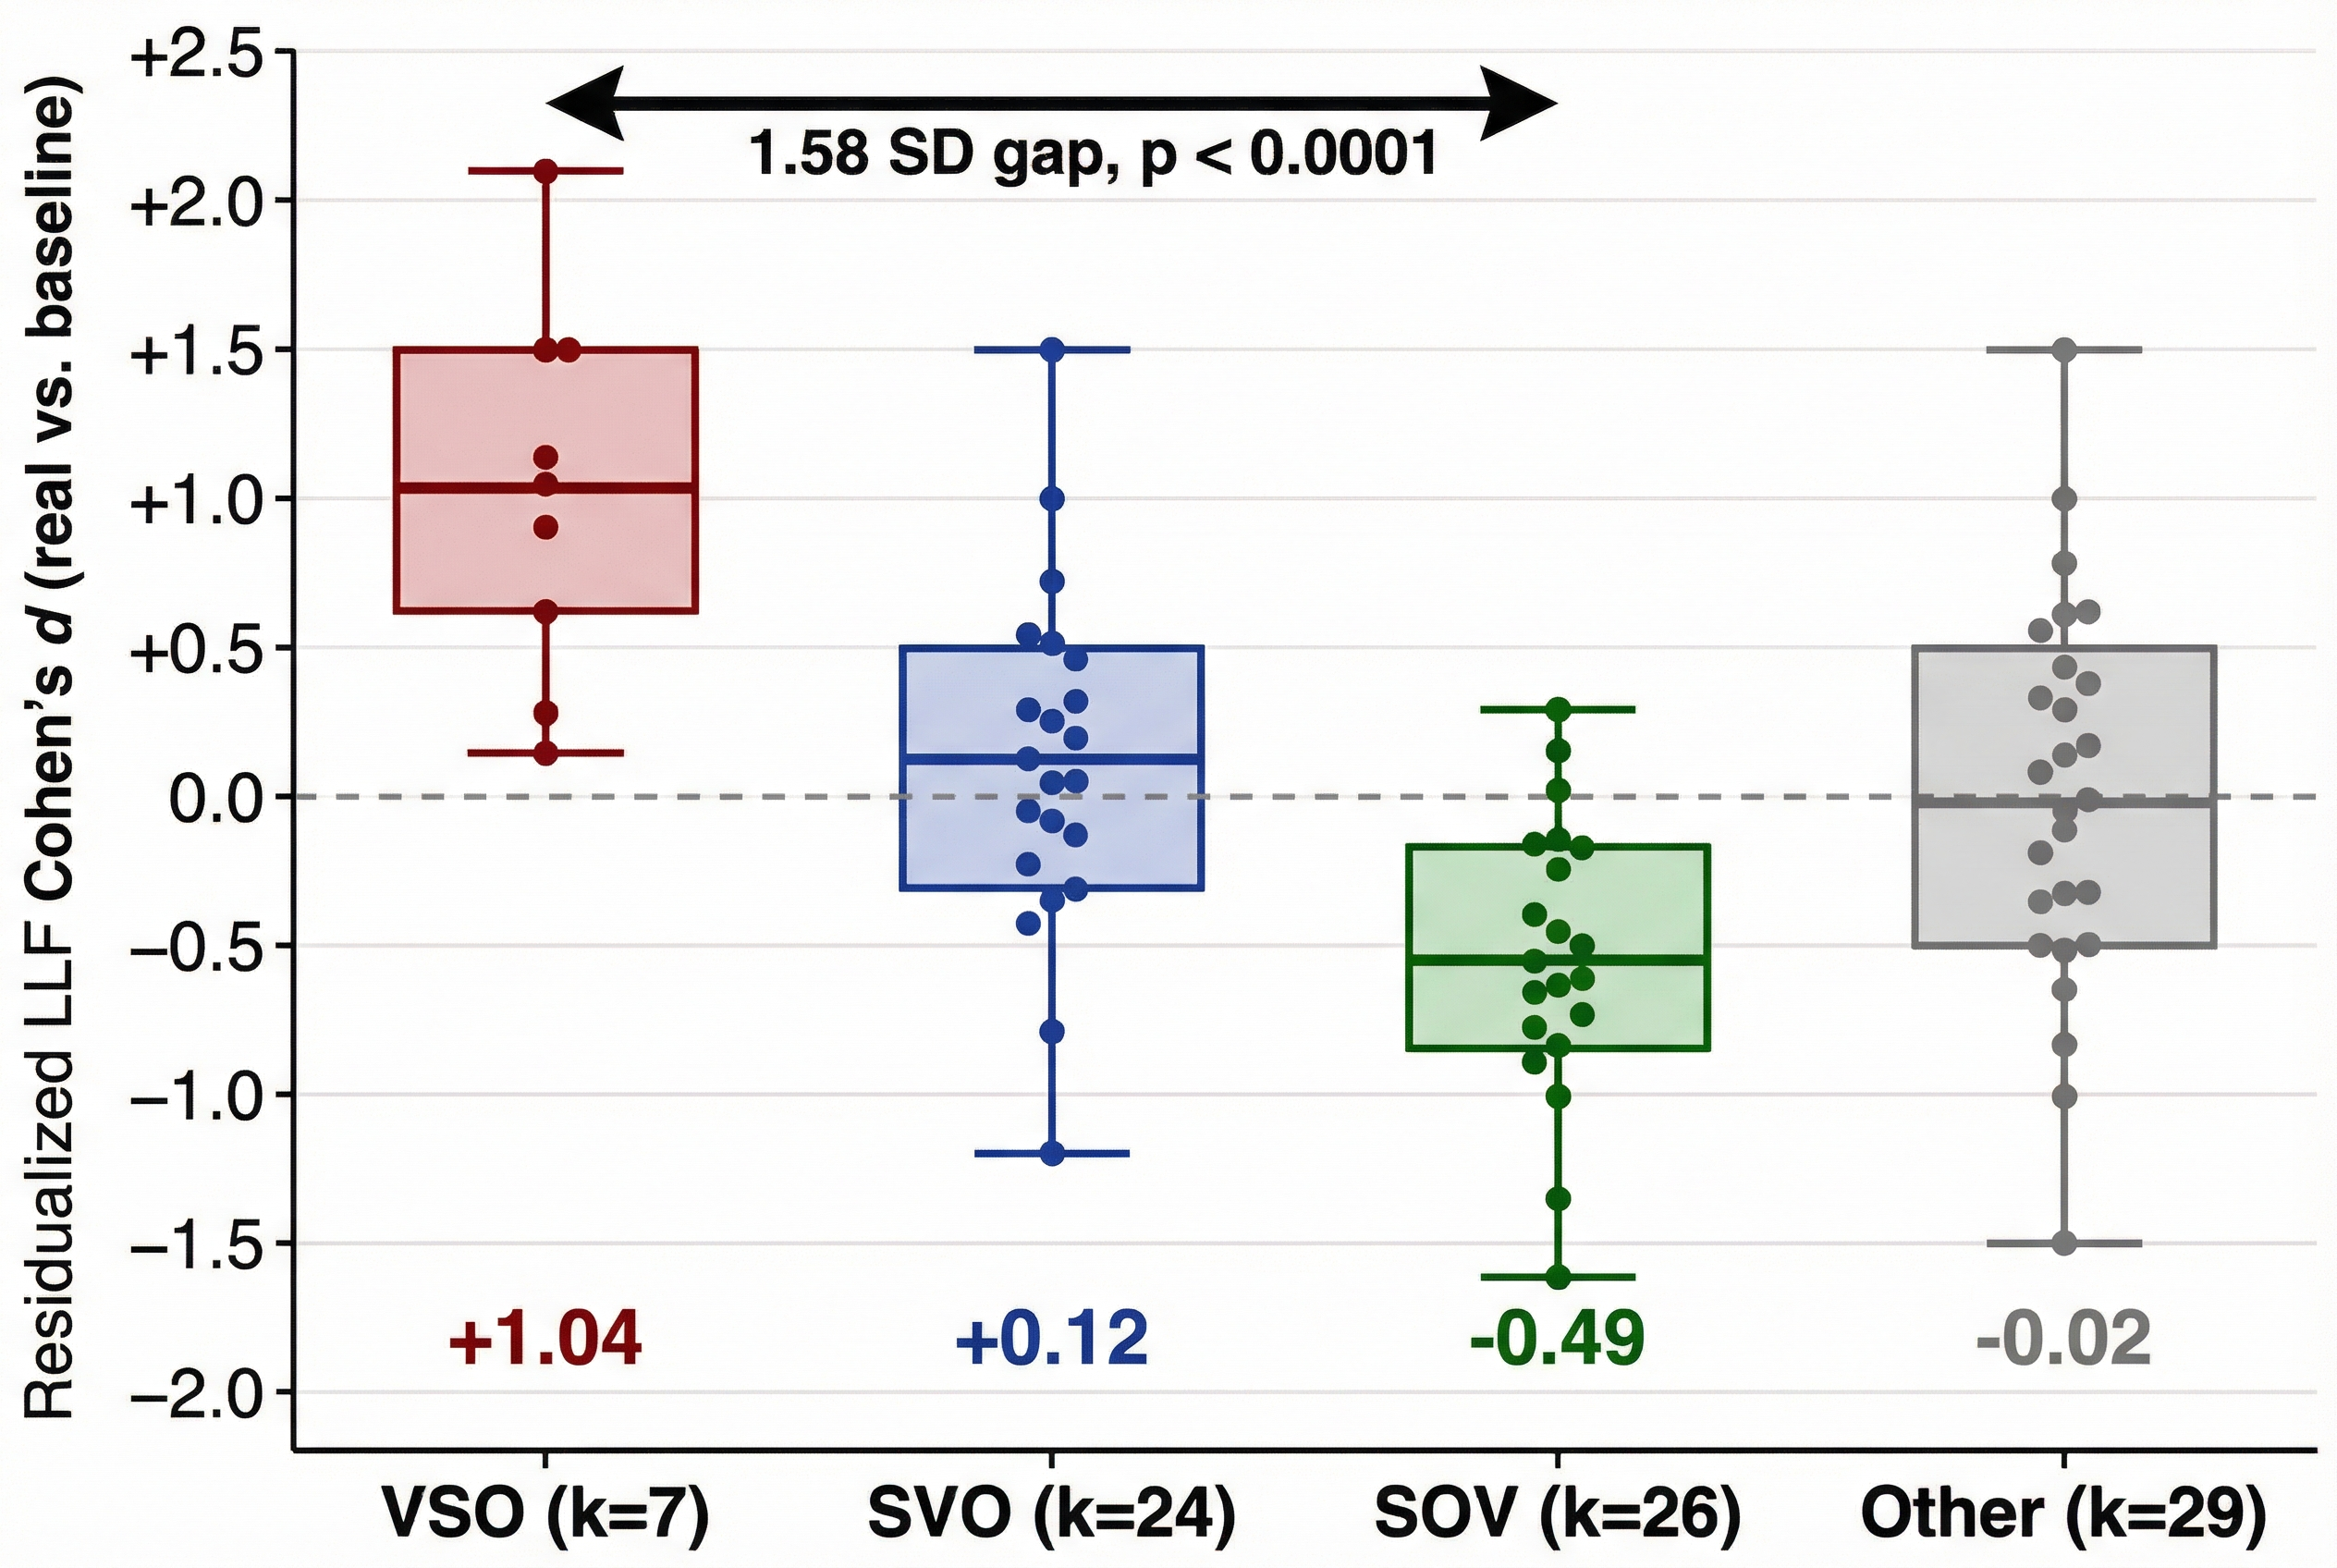
\includegraphics[width=0.92\textwidth,keepaspectratio]{figures/fig_typological_split_v0.png}
  \caption{Residualized LLF Cohen's $d$ (real vs.\ projective baselines) stratified by WALS word order across 86 treebanks. VSO languages show robust load smoothing (pooled $d = +1.04$, 95\% CI [0.79, 1.28], $k=7$), SVO languages show modest smoothing ($d = +0.12$, CI [$-0.01$, 0.26], $k=24$), SOV languages show anti-smoothing ($d = -0.49$, CI [$-0.61$, $-0.36$], $k=26$), and other/unclassified show near-zero effect ($d = -0.02$, $k=29$). The 1.58 SD VSO--SOV gap is significant by permutation test ($p < 0.0001$, 10,000 iterations). All pairwise Mann-Whitney tests are significant after Bonferroni correction.}
  \label{fig:typological_split}
\end{figure}

\paragraph{Permutation test.} Because the typological split was not pre-registered, we validated the 1.58~SD VSO--SOV gap with a 10,000-iteration permutation test that randomly reassigned word-order labels to treebanks. The observed gap exceeds all 10,000 permutations ($p < 0.0001$), and the Kruskal--Wallis $H$ statistic is also significant at $p < 0.0001$. All pairwise Mann--Whitney tests are significant after Bonferroni correction: VSO vs.\ SOV ($U = 182$, $p < 10^{-6}$), VSO vs.\ SVO ($U = 165$, $p < 10^{-5}$), SVO vs.\ SOV ($U = 557$, $p < 10^{-5}$)\footnote{Code: \url{https://github.com/AMGrobelnik/ai-invention-e4150b-head-directionality-dependent-temporal-d/tree/main/evaluation_iter3_typological_spl}}.

\paragraph{Head-final proportion as a continuous predictor.} The proportion of head-final dependencies in each treebank correlates strongly with residualized LLF Cohen's $d$ across all 86 treebanks: Pearson $r = -0.80$ ($p < 10^{-20}$, bootstrap 95\% CI [$-0.86$, $-0.71$]), partial $r = -0.80$ controlling for treebank size. The correlation explains the typological gradient more parsimoniously than the categorical word-order classification.

\paragraph{VSO robustness: expanded analysis and leave-one-out sensitivity.} The original Phase~2 VSO finding rested on only 7 treebanks at 500-sentence cap. We expanded to 11 VSO treebanks at 10,000-sentence cap, spanning 4 language families: Afro-Asiatic (Arabic PADT $d = 1.35$, Arabic PUD $d = 1.09$), Austronesian (Cebuano $d = 0.27$, Tagalog TRG $d = 2.34$, Tagalog Ugnayan $d = 0.53$), Indo-European (Irish Cadhan $d = 1.26$, Irish IDT $d = 1.42$, Irish TwittIrish $d = 0.90$, Scottish Gaelic $d = 0.51$, Welsh $d = 0.52$), and Tupian (Guajaj\'{a}ra $d = 1.06$). All 11 treebanks show positive Cohen's $d$ (11/11), with median $d = +1.06$.

\begin{figure}[!htbp]
  \centering
  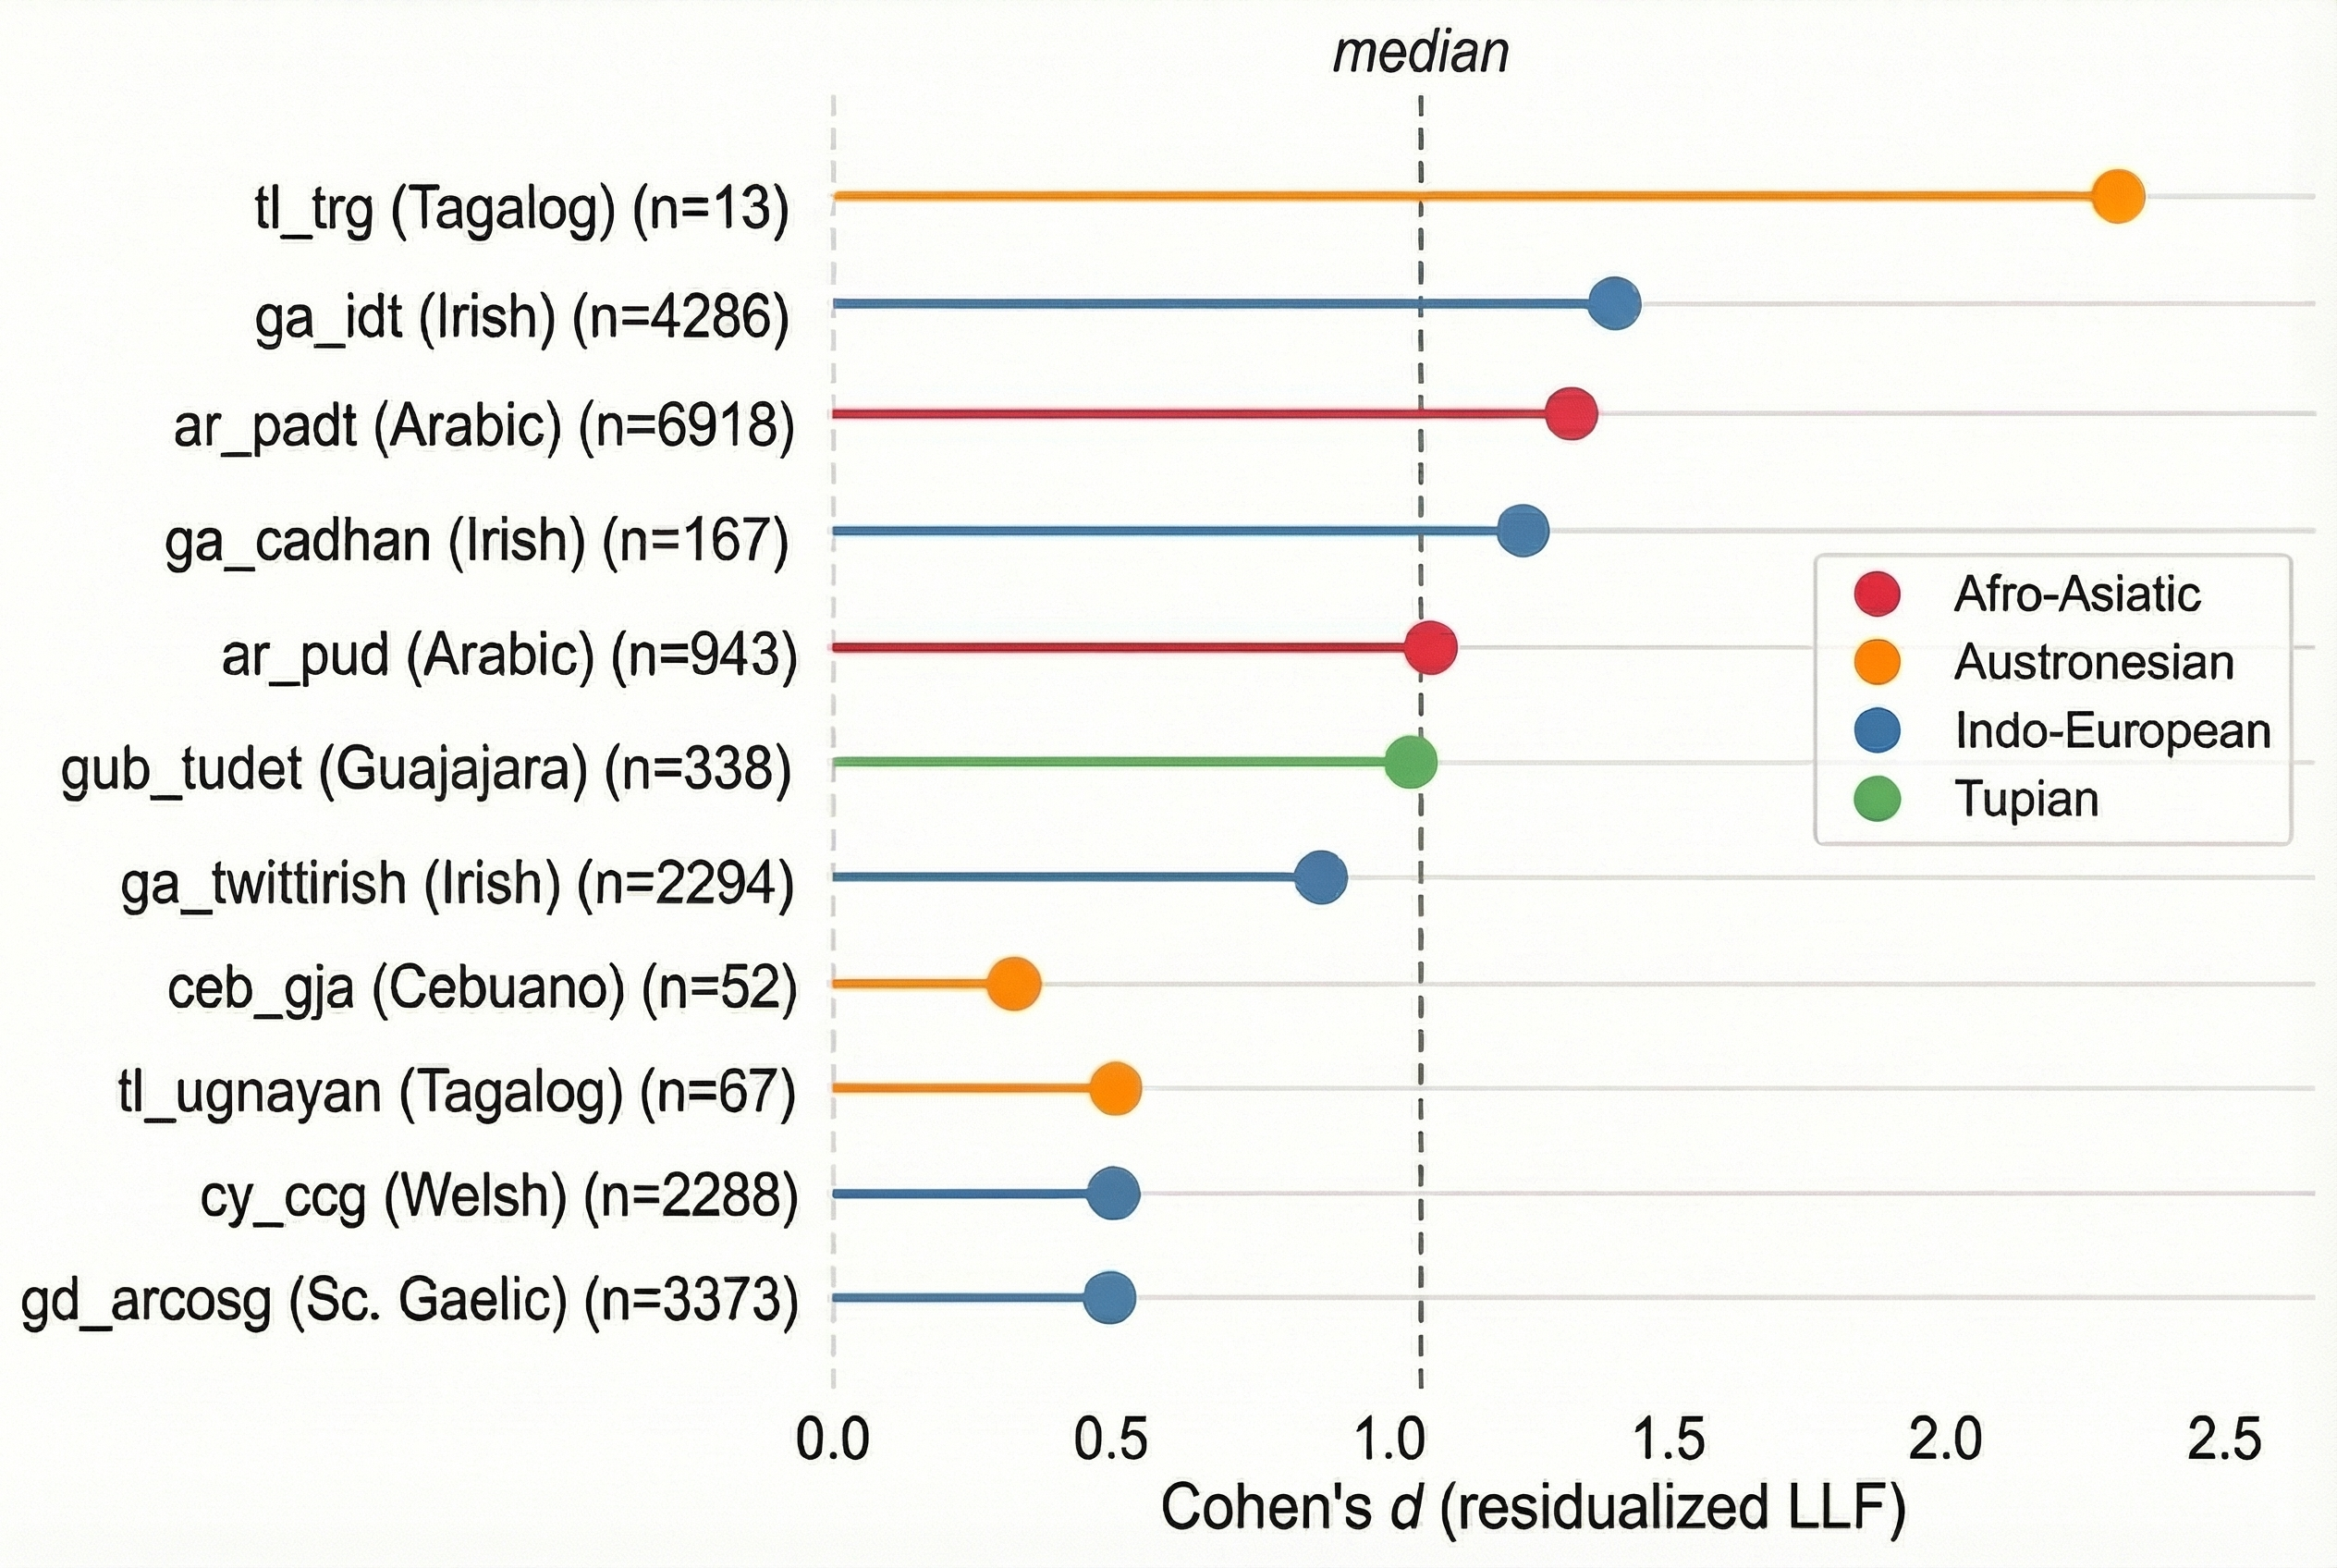
\includegraphics[width=0.92\textwidth,keepaspectratio]{figures/fig_vso_detail_v0.png}
  \caption{Individual Cohen's $d$ values for residualized LLF (real vs.\ projective baselines) across all 11 VSO treebanks, colored by language family. All 11 treebanks show positive $d$, spanning 4 families: Afro-Asiatic (Arabic PADT $d=1.35$, Arabic PUD $d=1.09$), Austronesian (Cebuano $d=0.27$, Tagalog TRG $d=2.34$, Tagalog Ugnayan $d=0.53$), Indo-European (Irish Cadhan $d=1.26$, Irish IDT $d=1.42$, Irish TwittIrish $d=0.90$, Scottish Gaelic $d=0.51$, Welsh $d=0.52$), and Tupian (Guajaj\'{a}ra $d=1.06$). Leave-one-out analysis confirms robustness: maximum median change is 0.08, with zero sign flips.}
  \label{fig:vso_detail}
\end{figure}

Leave-one-out analysis confirms robustness: removing any single treebank changes the VSO median $d$ by at most 0.08 (removing Arabic PADT), with zero sign flips. The minimum VSO--SOV gap across all leave-one-out iterations is 1.54~SD, and all leave-one-out permutation tests remain significant ($p < 0.001$). The effect is not driven by Arabic alone: removing both Arabic treebanks yields median $d = 0.98$ across the remaining 9 treebanks spanning 3 families.

\paragraph{Assessment of pre-registered predictions.} The pre-registered prediction that 70\% or more of treebanks would show significantly higher residualized LLF than baselines ($d > 0.2$) is not met: only 31.4\% exceed this threshold. The overall pooled effect is non-significant ($p = 0.53$). The typological split emerged from exploratory analysis and should be treated as hypothesis-generating rather than confirmatory. The permutation test provides protection against Type~I error for this specific post-hoc pattern, but replication on independent data remains necessary.


\subsection{Phase 3: $R^2$ Gap Decomposition Across Convexity Levels}
\label{sec:r2gap}

The proportion of processing cost explained by DD features decreases monotonically with $\alpha$ for both real and baseline sentences. However, this monotonicity is partly a mathematical consequence: at $\alpha = 1$, cost equals total IMB, which is a function of DD moments by Theorem~\ref{thm:decomposition}, guaranteeing high $R^2$. At higher $\alpha$, cost depends increasingly on the IMB profile peak by construction.

The empirically informative test compares the $R^2$ from DD features between real sentences and projective baselines at each $\alpha$ level\footnote{Code: \url{https://github.com/AMGrobelnik/ai-invention-e4150b-head-directionality-dependent-temporal-d/tree/main/evaluation_iter3_r_gap_decomposi}}. If the monotonic $R^2$ decrease were purely mathematical, the gap ($\Delta R^2 = R^2_{\text{real}} - R^2_{\text{baseline}}$) would remain constant across $\alpha$:

\begin{table}[!htbp]
\centering
\caption{$R^2$ from DD features for real sentences vs.\ projective baselines at each convexity exponent $\alpha$.}
\label{tab:r2gap}
\begin{tabular}{@{}lccc@{}}
\toprule
$\alpha$ & $R^2_{\text{real}}$ & $R^2_{\text{baseline}}$ & $\Delta R^2$ \\
\midrule
1.0 & 0.821 & 0.862 & $-0.040$ \\
1.2 & 0.750 & 0.795 & $-0.045$ \\
1.5 & 0.671 & 0.689 & $-0.018$ \\
2.0 & 0.602 & 0.533 & $+0.069$ \\
3.0 & 0.560 & 0.320 & $+0.240$ \\
\bottomrule
\end{tabular}
\end{table}

\begin{figure}[!htbp]
  \centering
  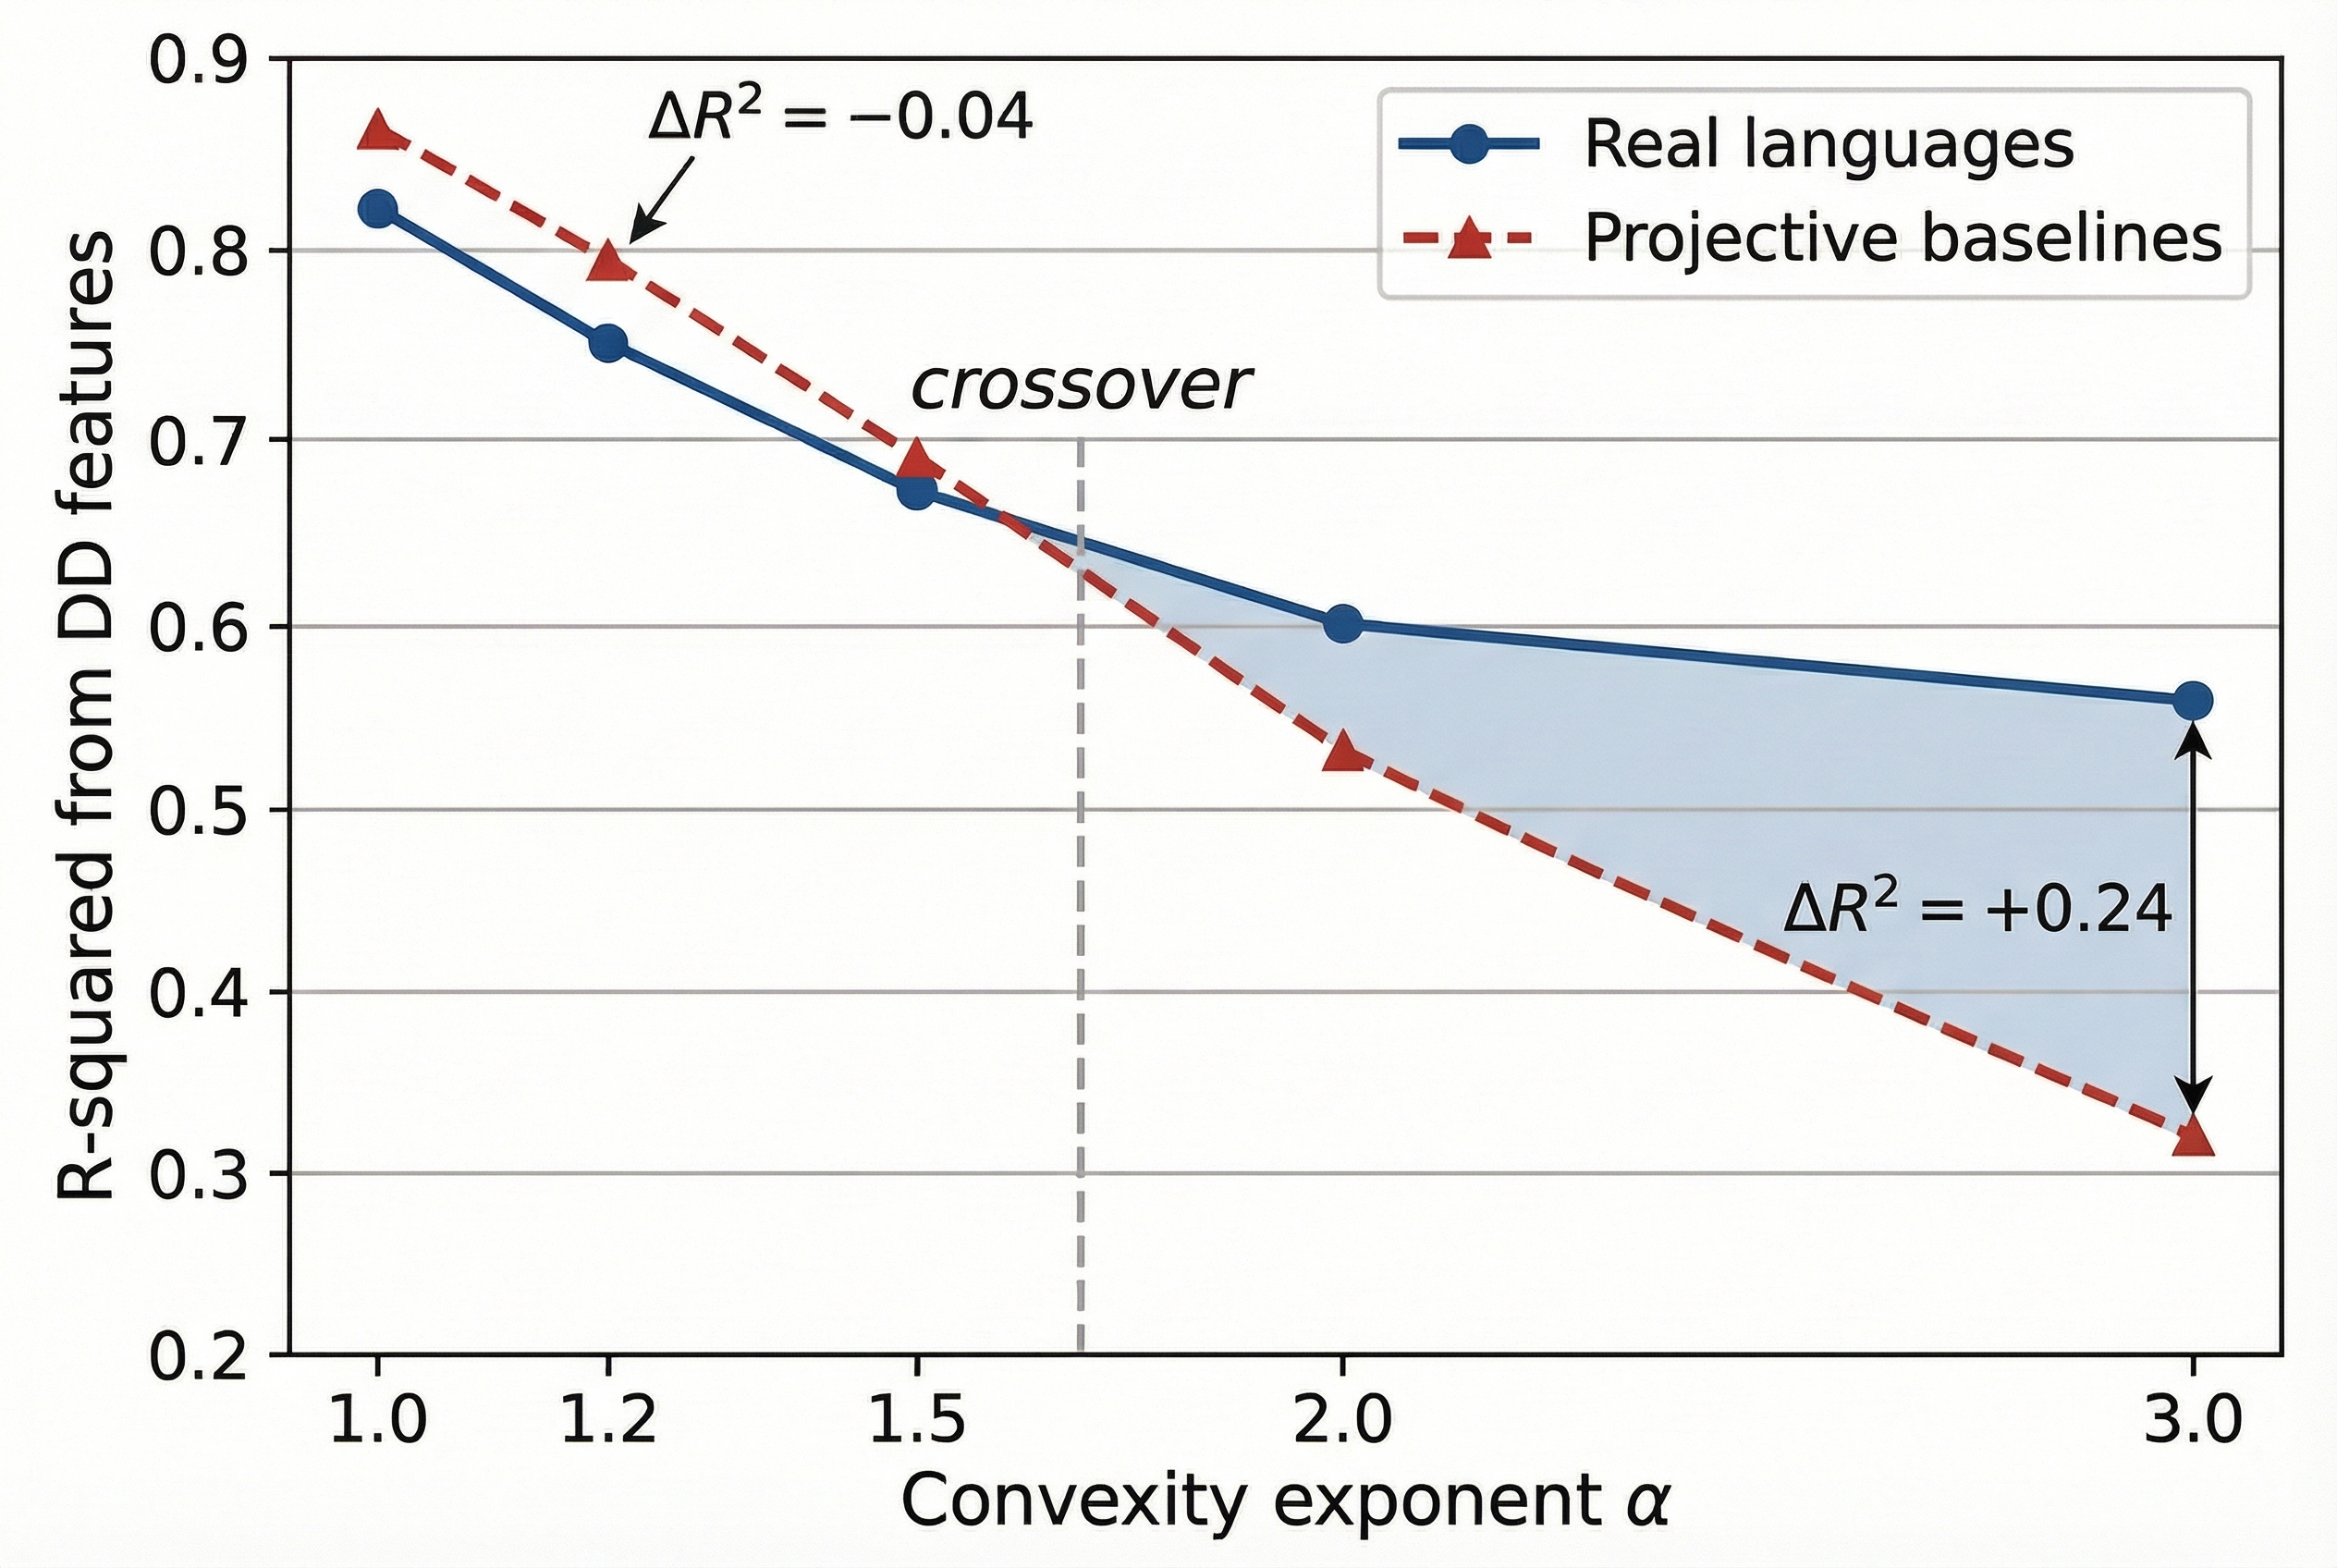
\includegraphics[width=0.92\textwidth,keepaspectratio]{figures/fig_r2_gap_v0.png}
  \caption{R-squared from DD features (6 predictors) for real sentences (solid line) and projective baselines (dashed line) at each convexity exponent $\alpha$. Both decrease with $\alpha$, but baseline $R^2$ drops faster: $\Delta R^2$ shifts from $-0.04$ at $\alpha=1$ to $+0.24$ at $\alpha=3$ (Spearman $\rho = 0.9$, $p = 0.037$). At high convexity, real languages retain systematically more DD-predictable cost structure than random baselines, ruling out a pure mathematical artifact in the $R^2$ monotonicity.}
  \label{fig:r2_gap}
\end{figure}

The $\Delta R^2$ increases monotonically from $-0.04$ to $+0.24$ (Spearman $\rho = 0.9$, $p = 0.037$). At low convexity ($\alpha \leq 1.5$), baselines have higher $R^2$ than real sentences, meaning DD features explain baseline cost structure better---consistent with baselines being determined largely by DD moments. At high convexity ($\alpha \geq 2.0$), the relationship reverses: real languages retain systematically more DD-predictable cost structure than random baselines. The $\Delta R^2$ range of 0.28 across $\alpha$ levels rules out the pure mathematical artifact hypothesis: if $R^2$ monotonicity were entirely mechanical, the gap would be constant.

The residualized convexity Cohen's $d$ values (comparing real vs.\ baseline cost after controlling for DD features) are uniformly weak and do not increase monotonically with $\alpha$. The residualized negative control at $\alpha = 1.0$ yields $d = -0.085$, which is small but not the predicted zero. The originally claimed ``cleanest evidence'' from raw $R^2$ monotonicity is therefore substantially weaker than presented in the previous draft---the $R^2$ gap decomposition provides a more honest assessment.


\subsection{Phase 4: Intervener Complexity Independence}

Nested logistic regression models across 35 typologically diverse treebanks tested whether LLF and residualized $\max(\text{IMB})$ add explanatory power beyond IC\footnote{Code: \url{https://github.com/AMGrobelnik/ai-invention-e4150b-head-directionality-dependent-temporal-d/tree/main/experiment_iter2_phase_3_ic_inde}}. Adding IC to the DD-only model improved mean pseudo-$R^2$ from 0.1064 to 0.1475 ($\Delta = 0.041$). Adding LLF further improved to 0.1684 ($\Delta = 0.021$).

\paragraph{Per-treebank effects.} LLF significantly improved model fit beyond IC in 74.3\% of treebanks (Bonferroni-corrected $p < 0.05$). Residualized $\max(\text{IMB})$ was significant in 60.0\% of treebanks.

\paragraph{Meta-analysis.} DerSimonian--Laird random-effects meta-analysis yielded non-significant pooled effects: LLF pooled effect $= -0.047$ ($p = 0.589$), residualized $\max(\text{IMB})$ pooled effect $= -0.106$ ($p = 0.194$). The extreme heterogeneity ($I^2 > 97\%$) reflects the direction-varying nature of LLF effects across word-order types, consistent with the typological split. The bidirectional test confirms IC remains highly significant after controlling for LLF (pooled effect $= -1.743$, $p < 10^{-6}$), indicating IC and temporal overlap capture partially independent signals.

The Phase~4 results are inconclusive for the pooled independence claim: temporal overlap adds meaningful per-treebank information beyond IC, but the direction-varying nature across typological groups prevents a clean aggregate signal.


\subsection{Phase 5: IMB Variants and Head-Directionality}
\label{sec:imb_variants}

\paragraph{Three IMB variants.} We computed three IMB variants across 21 treebanks (11 VSO, 5 SOV, 5 SVO), each compared against 100 projective baselines:

\begin{enumerate}
  \item \emph{Standard IMB}: all dependencies across their full span with age from span start.
  \item \emph{Head-initial-only IMB} (Definition~\ref{def:hio}): only head-initial dependencies, full span, age from span start.
  \item \emph{True encounter-only IMB}: restricting to positions where both endpoints have been encountered, with age from the later encounter.
\end{enumerate}

The true encounter-only IMB is identically zero for every sentence across all 25,739 sentences analyzed. At any position $j$ where both a dependent $i$ and its head $h(i)$ have been encountered, the dependency is already resolved---the span endpoint has been reached and no open dependency remains. IMB burden is therefore entirely anticipatory: generated by dependencies whose heads (or dependents) have not yet appeared.

\paragraph{Head-initial-only amplifies the typological gradient.} The head-initial-only variant amplifies the VSO--SOV gradient: VSO median $d = +1.48$ (vs.\ $+1.06$ standard), SVO median $d = +0.68$ (vs.\ $+0.17$), SOV median $d = -1.05$ (vs.\ $-0.79$). The VSO--SOV gap widens from 1.85 to 2.53~SD. For SOV languages, excluding head-final dependencies (the majority) amplifies the anti-smoothing signal because the remaining head-initial dependencies in SOV languages cluster in unusual configurations relative to baselines.

\begin{figure}[!htbp]
  \centering
  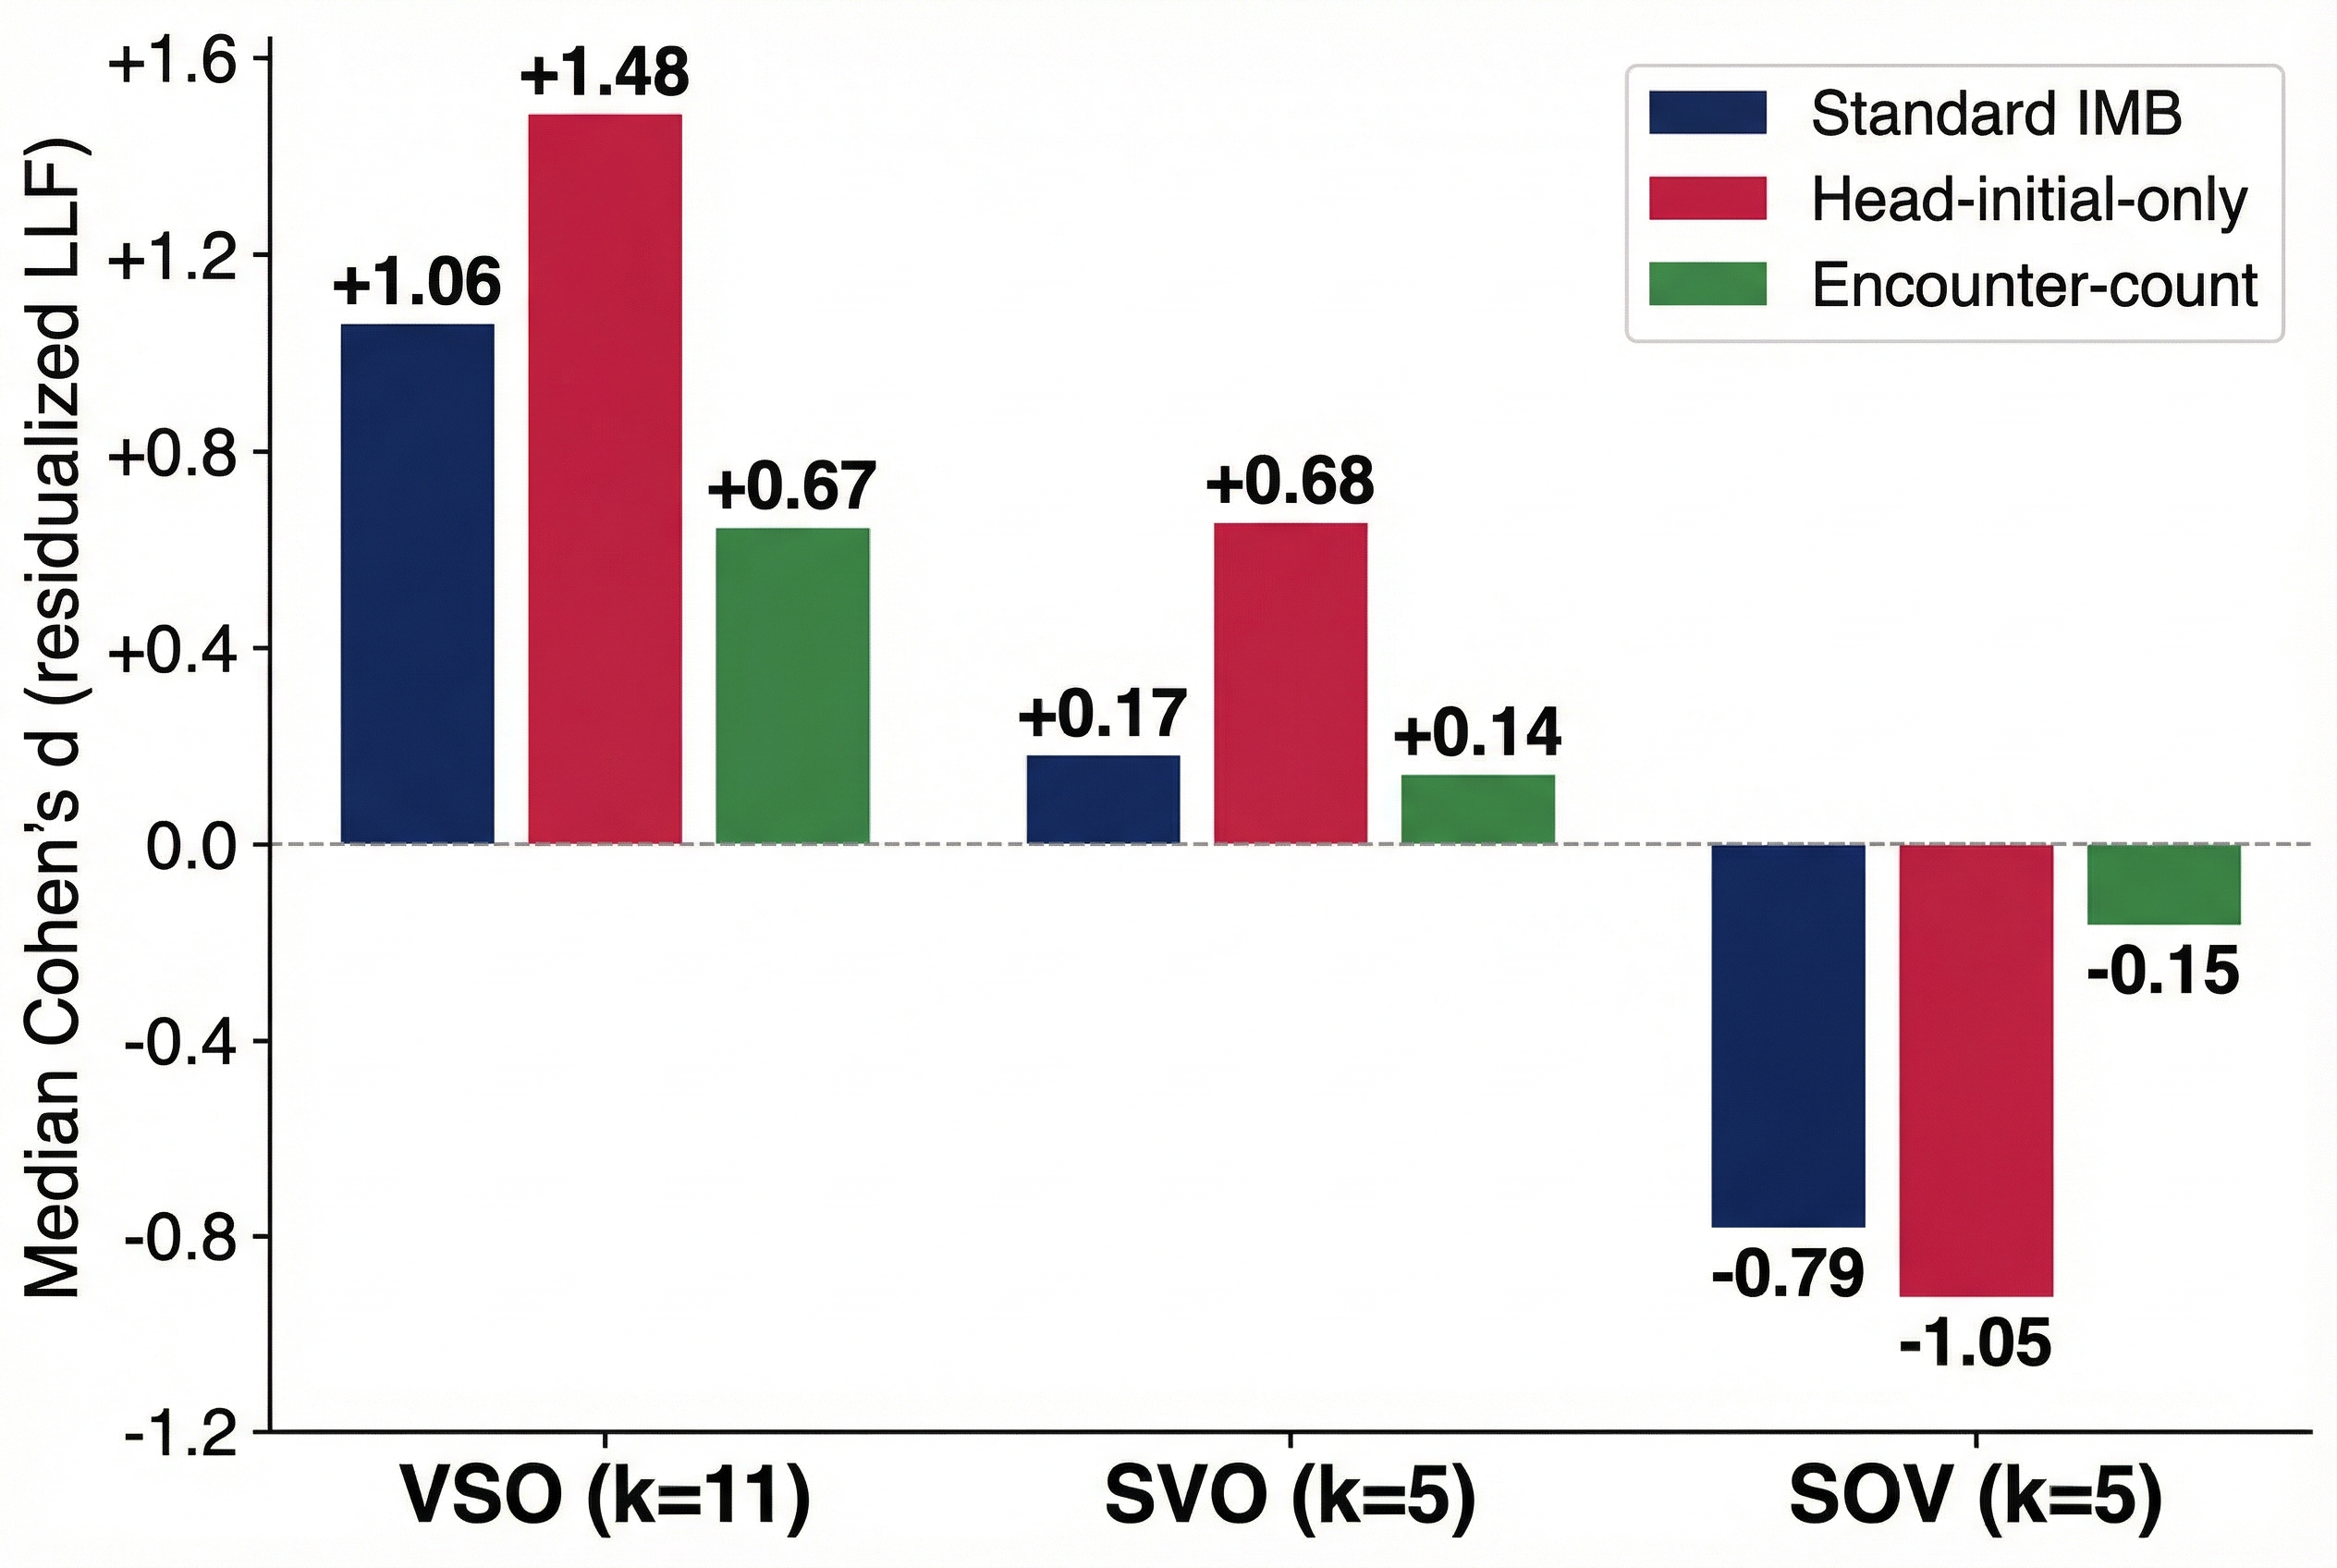
\includegraphics[width=0.92\textwidth,keepaspectratio]{figures/fig_imb_variants_v0.png}
  \caption{Median Cohen's $d$ for residualized LLF (real vs.\ baselines) under three IMB computation variants across VSO ($k=11$), SVO ($k=5$), and SOV ($k=5$) treebanks. Standard IMB shows the typological gradient (VSO $d=+1.06$, SOV $d=-0.79$). Head-initial-only IMB amplifies the gradient (VSO $d=+1.48$, SOV $d=-1.05$). Encounter-count LLF (counting dependencies with both endpoints encountered, without age-weighting) compresses the SOV anti-smoothing ($d=-0.15$) while preserving VSO smoothing ($d=+0.67$), confirming the SOV pattern is driven by head-final dependency accumulation.}
  \label{fig:imb_variants}
\end{figure}

\paragraph{Encounter-count LLF.} As an intermediate variant, encounter-count LLF counts how many dependencies have both endpoints encountered at each position (without age-weighting). VSO languages show $d = +0.67$ for encounter-count LLF---positive and substantial, though smaller than the standard LLF effect ($d = +1.06$). SOV languages show $d = -0.15$---negative but much closer to zero than the standard variant ($d = -0.79$), confirming that the SOV anti-smoothing effect is largely driven by the accumulation of head-final dependencies awaiting verb encounter.


\subsection{Phase 6: Spoken-Written Modality and Case-Marking}

Six spoken-written treebank pairs were analyzed with disfluency-specific dependency relations excluded\footnote{Code: \url{https://github.com/AMGrobelnik/ai-invention-e4150b-head-directionality-dependent-temporal-d/tree/main/experiment_iter2_modality_head_f}}. Three of six pairs showed spoken higher residualized LLF (Slovenian $d = 0.031$, Turkish $d = 0.121$, English $d = 0.027$), while three showed spoken lower (French $d = -0.531$, Italian $d = -0.181$, English ESL $d = -0.243$). The pre-registered prediction of 60\% or more pairs showing spoken-higher is not met (3/6 $= 50\%$). Genre and register confounds between treebank pairs---particularly the French comparison (narrative ParisStories vs.\ formal GSD)---likely dominate the modality signal. With only six pairs, the analysis lacks the power to isolate a reliable modality effect.

Among 51 SOV treebanks, no significant correlation was found between morphological case richness and LLF ($r = -0.047$, $p = 0.74$). Differential object marking analysis across 22 treebanks yielded 9 of 22 showing case-marked sentences with higher LLF, and the mixed-effects coefficient was non-significant ($\beta = -0.0006$, $p = 0.20$). The case-marking hypothesis is not supported.


%% ============================================================
\section{Related Work}
\label{sec:related}
%% ============================================================

\subsection{Dependency Distance Minimization}

Gibson's Dependency Locality Theory \citep{Gibson1998, Gibson2000} established that processing difficulty increases with linear distance between syntactically related words. \citet{Futrell2015} provided foundational large-scale evidence across 37 languages. \citet{Liu2008} analyzed 20 languages, and \citet{Temperley2018} reviewed DDM as a potential universal. The DDM consensus was disrupted by \citet{Yadav2022}, who showed across 54 SUD treebanks that DDM effects vanish when IC and tree topology are jointly controlled. \citet{Dyer2023} replicated the finding on 35 languages, and \citet{Aggarwal2025} established IC as a structurally grounded measure with explanatory power beyond linear distance.

The present work addresses the puzzle raised by Yadav et al.\ by proposing temporal load distribution as a distinct dimension of syntactic organization. Our Phase~4 results find that LLF adds incremental power beyond IC per-treebank (74.3\% significant), but the effect direction varies across languages, preventing a clean pooled signal. The typological split suggests that temporal overlap and IC interact with head-directionality in ways that pooled analysis obscures.

\subsection{Per-Position Memory Models}

Gibson's 1998 SPLT \citep{Gibson1998} originally included locality in storage cost---older predictions cost more---but the 2000 DLT revision \citep{Gibson2000} explicitly removed age-sensitivity, defining storage cost as a binary count of predicted heads. \citet{Chen2005} validated binary counting experimentally and found that storage duration had no significant effect on reading times. Our sentence-length-stratified analysis shows that while proportional $R^2$ from DD moments increases with sentence length, absolute residual variance also grows substantially (from 5.4 at 8--12 words to 224.5 at 36+ words). The length-stratification result does not support the ``limited power from short sentences'' explanation for the Chen et al.\ null, leaving the tension between age-weighted IMB and duration-insensitive reading times as an open question.

\citet{Kobele2013} introduced stack tenure for Minimalist Grammar parsers, and \citet{Graf2017} formalized tenure, payload, and size as separate dimensions. IMB combines tenure and payload into a single age-weighted sum computed directly from dependency trees without requiring grammar-specific parsers---a practical advantage for cross-linguistic corpus studies.

\subsection{Information-Theoretic Approaches}

\citet{Clark2023} demonstrated cross-linguistic pressure for Uniform Information Density (UID) in word order. LLF and UID are conceptually parallel---both are uniformity hypotheses---but target fundamentally different quantities. UID optimizes surprisal uniformity (information-theoretic, requiring trained language models), while LLF optimizes memory burden uniformity (syntactic-structural, requiring only the dependency parse). A word can have low surprisal yet occur at a position with many concurrent open dependencies, and vice versa. \citet{Futrell2020a} unified surprisal and locality theories through lossy-context surprisal, and \citet{Xu2024} linked information-theoretic properties to dependency length.

\subsection{Annotation Framework Considerations}

Our use of UD treebanks differs from Yadav et al.'s \citep{Yadav2022} use of SUD. In UD, content words are always heads; in SUD, function words (auxiliaries, copulas, adpositions, subordinators) can be heads \citep{Gerdes2019}. Since IC counts intervening heads, IC values differ systematically between frameworks. Our Phase~4 results using UD-based IC may not be directly comparable to Yadav et al.'s SUD-based findings.


%% ============================================================
\section{Discussion}
\label{sec:discussion}
%% ============================================================

\subsection{The Typological Split as an Exploratory Finding}

The most striking result is a strong typological split in load-smoothing direction. VSO languages (pooled $d = +1.04$, 11 treebanks, 4 families) show robust load smoothing relative to projective baselines, SVO languages show modest non-significant smoothing ($d = +0.12$, 24 treebanks), and SOV languages show the opposite anti-smoothing pattern ($d = -0.49$, 26 treebanks). The VSO--SOV gradient spans 1.58 standard deviations and is confirmed by permutation testing ($p < 0.0001$) and leave-one-out sensitivity analysis.

The finding was not pre-registered and emerged from exploratory analysis. The permutation test provides protection against Type~I error for this specific pattern, and the leave-one-out analysis confirms that no single treebank drives the VSO effect. Nevertheless, the finding requires replication on independent data---particularly for VSO languages, where 11 treebanks from 4 families provide reasonable but not conclusive typological coverage. The effect is not driven by Arabic alone (removing both Arabic treebanks yields median $d = 0.98$ across 9 remaining treebanks), and the continuous correlation with head-final proportion ($r = -0.80$) suggests a gradient rather than categorical phenomenon.

\subsection{Anticipatory Load as the Mechanism}

The discovery that true encounter-only IMB is identically zero provides a mechanistic insight: all memory burden measured by IMB derives from anticipatory load---predictions about syntactic material that has not yet been encountered. In head-initial languages, the head appears first, immediately creating predictions for dependents that accumulate age as the sentence progresses. Load smoothing in VSO languages may reflect optimization of how these predictions are distributed across positions. In head-final languages, the verb appears last, creating a large pool of predicted-but-unseen heads that the standard IMB model counts as open dependencies accumulating burden. The head-initial-only variant, which excludes these pending predictions, reduces peak IMB by 67--85\% in SOV languages, suggesting the SOV anti-smoothing pattern reflects the cognitive asymmetry between anticipatory and resolution-based processing rather than genuine lack of load optimization.

The finding aligns with antilocality effects documented by \citet{Konieczny2000} and \citet{Vasishth2003}, where pre-verbal arguments facilitate rather than hinder verb processing in head-final languages, and with expectation-based accounts \citep{Levy2008} where predicted material generates facilitation rather than burden.

\subsection{$R^2$ Gap Decomposition and Convexity}

The $R^2$ gap decomposition provides a more nuanced assessment of convexity evidence than the raw $R^2$ monotonicity reported previously. The key finding is that $\Delta R^2$ (real minus baseline) shifts from negative at low convexity to positive at high convexity (Spearman $\rho = 0.9$, $p = 0.037$). At $\alpha = 3$, real languages show $R^2 = 0.560$ while baselines show $R^2 = 0.320$---a gap of $+0.24$, meaning real languages retain substantially more DD-predictable cost structure. The reversal at $\alpha \sim 1.5$--$2.0$ suggests an empirical threshold where temporal arrangement in real languages diverges from random baselines, consistent with the ACT-R fan effect prediction of $\alpha \sim 1.5$--$2.0$ \citep{Lewis2005}.

However, the residualized convexity analysis (comparing real vs.\ baseline after DD controls) yields uniformly weak effects that do not follow the predicted monotonic pattern. The evidence for convex cost is therefore suggestive rather than conclusive: real languages organize temporal load differently from baselines in ways that matter more at higher convexity, but the signal is modest after controlling for DD features.

\subsection{Honest Assessment of Pre-Registered Predictions}

Against the pre-registered success criteria\footnote{Code: \url{https://github.com/AMGrobelnik/ai-invention-e4150b-head-directionality-dependent-temporal-d/tree/main/evaluation_iter3_comprehensive_h}}: (1)~The prediction that 70\% or more of treebanks show $d > 0.2$ is not met (31.4\%). (2)~The $R^2$ novelty test partially passes: standard $R^2 = 0.948$ exceeds 0.90, but head-initial-only $R^2 = 0.883$ falls below it. (3)~The IC independence test is inconclusive (74.3\% per-treebank significant, but meta-analysis non-significant). (4)~The spoken-written prediction is not met (3/6 pairs). (5)~Case-marking predictions are null. The overall scorecard is 0 confirmed, 1 partial pass, 1 weak pass, 1 inconclusive, 4 failures.

The exploratory typological split, validated by permutation testing and sensitivity analysis, is the primary contribution. The paper's value lies not in confirming universal load smoothing but in identifying a typologically structured pattern that connects head-directionality to temporal dependency organization---a relationship invisible to aggregate DD statistics.

\subsection{Limitations}

Several limitations qualify the findings. First, the 5.25\% residual variance in standard $\max(\text{IMB})$ is modest, though comparable to other secondary optimization pressures. Second, the UD annotation framework differs from SUD used by \citet{Yadav2022}, and IC values differ systematically between frameworks. Third, the head-initial-only IMB variant (Definition~\ref{def:hio}) is an approximation whose cognitive interpretation---that predicted-but-unseen heads impose zero memory cost---is likely too extreme. A graded model where predicted heads impose partial cost, with the partial weight estimated from reading-time data, would be more realistic. Fourth, the sentence-length-stratified analysis does not support the dismissal of the \citet{Chen2005} null result on storage duration, leaving a tension between the age-weighting premise and experimental evidence. Fifth, with only 11 VSO treebanks from 4 families, the typological coverage for the strongest finding remains limited.


%% ============================================================
\section{Conclusion}
\label{sec:conclusion}
%% ============================================================

We introduced Instantaneous Memory Burden as an age-weighted generalization of Gibson's DLT storage cost and identified peak IMB as a metric capturing temporal dependency overlap invisible to aggregate DD statistics. The 5.25\% residual variance in $\max(\text{IMB})$ beyond DD moments---comparable in magnitude to heavy-NP shift and given-before-new ordering effects---drives a typologically structured pattern: VSO languages smooth temporal load relative to projective baselines (pooled $d = +1.04$, 11 treebanks, 4 families), SVO languages show modest smoothing ($d = +0.12$), and SOV languages show anti-smoothing ($d = -0.49$). The 1.58~SD VSO--SOV gradient is confirmed by permutation testing ($p < 0.0001$) and robust to leave-one-out sensitivity analysis.

The discovery that true encounter-only IMB is identically zero establishes that all measured burden derives from anticipatory load---predictions about unseen syntactic material. The head-initial-only variant explains the SOV anti-smoothing pattern through the cognitive asymmetry between prediction and resolution in head-final languages.

The typological split is an exploratory finding that requires replication. Future work should pursue three directions:

\begin{itemize}
  \item Developing a graded encounter model where predicted-but-unseen heads impose partial rather than zero cost, with the partial weight estimated from reading-time data.
  \item Replicating the IC independence test using SUD treebanks to ensure comparability with \citet{Yadav2022}.
  \item Testing whether residualized $\max(\text{IMB})$ predicts online processing difficulty in eye-tracking corpora beyond what DD and IC predict, providing direct psycholinguistic validation of the age-weighting premise that the \citet{Chen2005} null result challenges.
\end{itemize}


%% ============================================================
\bibliography{references}
%% ============================================================

\end{document}
